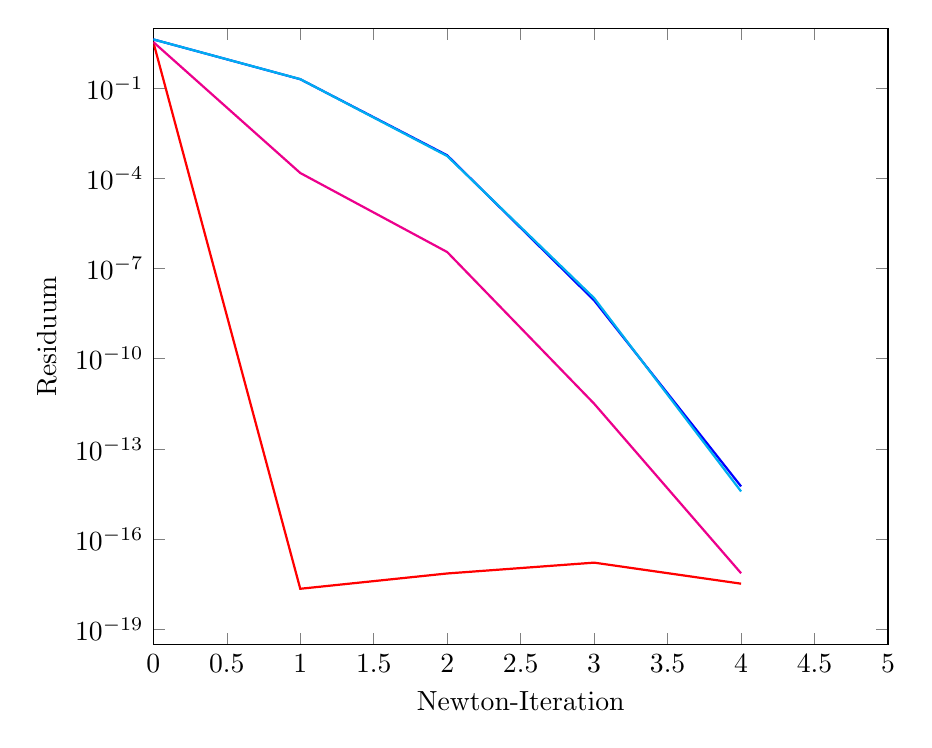
\begin{tikzpicture}[every plot/.append style={thick}] 
\begin{axis}[ 
label style={font=\normalsize}, 
xlabel={Newton-Iteration}, 
ylabel={Residuum}, 
xmin=0, xmax=5, 
ymode=log, 
ymin=0, ymax=10, 
width=0.9\textwidth, 
grid style=dashed, 
] 
\addplot[ 
color=blue, 
] 
coordinates { 
(0, 4.25e+00)(1, 2.01e-01)(2, 5.89e-04)(3, 8.72e-09)(4, 5.61e-15)}; 
\addplot[ 
color=red, 
] 
coordinates { 
(0, 3.47e+00)(1, 2.20e-18)(2, 7.11e-18)(3, 1.63e-17)(4, 3.25e-18)}; 
\addplot[ 
color=cyan, 
] 
coordinates { 
(0, 4.25e+00)(1, 2.02e-01)(2, 5.56e-04)(3, 1.04e-08)(4, 3.81e-15)}; 
\addplot[ 
color=magenta, 
] 
coordinates { 
(0, 3.47e+00)(1, 1.52e-04)(2, 3.55e-07)(3, 3.18e-12)(4, 7.22e-18)}; 
\end{axis} 
\end{tikzpicture} 
